\documentclass[10pt,a4paper]{article}
\usepackage[latin1]{inputenc}
\usepackage{amsmath}
\usepackage{amsfonts}
\usepackage{hyperref}
\usepackage{amssymb}
\usepackage{graphicx}
\usepackage{kpfonts}
\usepackage{csvsimple}
\usepackage[numbers]{natbib}
\usepackage{listings}
\usepackage{subfigure}
\usepackage{graphicx}
\usepackage{mathtools}
\DeclarePairedDelimiter\ceil{\lceil}{\rceil}
\DeclarePairedDelimiter\floor{\lfloor}{\rfloor}
%Styles and setups
\graphicspath{{./images/}}

\title{Activity prediction using hybrid generative/discriminative model}
\author{Lio Enrico 822861, Vasquez Alessandro 822569}
\begin{document}
	\maketitle
	\newpage
	\section{Introduction}
	\subsection{Objectives}
	In this work we want to explore the power of a particular machine learning's hybrid model, composed by a deep ANN (Artificial Neural Network) for the discriminative part and an HMM (Hidden Markov Model) for the generative part. In this hybrid model, the output of the ANN is used to refine the matrix of emission probabilities of the HMM so that the accuracy of the deep neural network is somehow ``transmitted'' to the HMM framework.
	\subsection{The setting}
	To train and test the hybrid model we used a dataset generated by a Wireless Sensor Network (WSN) which recorded the activation of almost a dozen sensors spread all over a user's home for almost a couple of weeks. The sensors' dataset is accompanied by another dataset created from the user's annotations about which ADL (activity of daily living) was executed during a given interval of time. By setting the sensors' recordings as the features and the user's ADL as the targets we can build a model that infers the sequence of ADL the user was executing by taking into consideration which sensors were activated during that period of time. 
	
	\section{Design choices}
	\subsection{Data parsing, data alignment, data mapping}
	In order to get a discretized temporal format of the dataset, we sliced the data in regularly spaced intervals of time. The chosen length of those intervals is $\Delta t=60s$.
	For each $\Delta t$, we consider the first ADL being executed in that interval, whereas for the sensors we consider all sensor that were activated at least once during the considered interval. The choice of excluding other ADLs that could possibly appears in the same $\Delta t$, was made by considering that if an ADL appears as the second activity during a given interval, two scenarios are possible: in the first one the ADL is so short that will not appear in the next time interval. In this case we assume that activity to be noise and do not consider it. In the second scenario the ADL is long enough to appear as the first ADL in the next interval, and will be associated to that interval. An example of these scenarios is illustrated in figure \ref{fig:intervals}. 
	\begin{figure}
		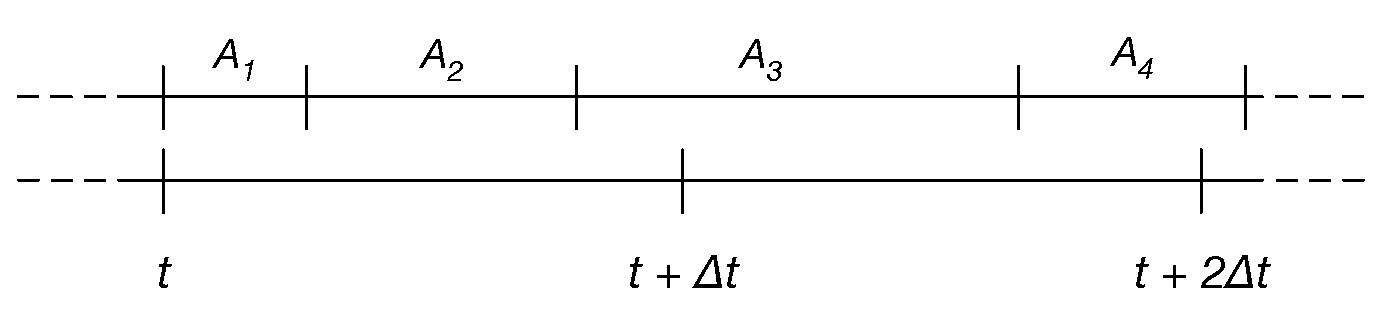
\includegraphics[ width=1.1\textwidth]{intervals.eps}
		\caption{ADLs and intervals. The activity $A_2$ being too short is considered noise and is dropped from the dataset. At the opposite, $A_3$  is long enough to be detected in the next interval.}
		\label{fig:intervals}
	\end{figure}
	We mapped each activity and each sensor into an integer number based on the order of appearance in the dataset, such that the first activity/sensor to appear in the dataset is mapped as the $0$-th activity/sensor. This means that the mapping differs for each different dataset. In our case, two datasets were used ($A$ and $B$), thus two different mappings have been produced: \\
	% mettere i csv coi mapping
	\begin{center}
		\csvautotabular{csvs/labels_states_A.csv}
		\csvautotabular{csvs/labels_states_B.csv}
	\end{center}
	
	
	A \textit{configuration}  is an array in which the $i$-th element is set to $1$ if the $i$-th sensor was activated during the given interval of time, 0 otherwise. Each configuration is associated with the ADL the user was executing during that interval of time, and is used as a single observation by the model.
	
	
	\section{Hybrid model}
	\subsubsection{Neural Network}
	The neural network takes the configuration $y_t$ associated to the time interval $t$ as its input whereas the final output $\sigma(\bf o \rm)$, in accordance to our model, corresponds to the probability for the configuration $y_t$ to be observed given the state $x_{i_t}$, i.e. $\sigma(o_i) = p( y_t\ |\ x_{i_t}),$ for each possible state $i$ at the time $t$\footnote{In the original paper  the author used the Bayes rule on the output of the softmax function \cite{DBLP:journals/eswa/OrdonezITLS13} since they considered it the probability $p(\vec x_t\ |\ y_t)$. We made a different choice in order to not ``contaminate'' the neural network's result with the a priori probabilities of features and targets.}, where $\sigma$ is the softmax function. $\sigma$ transforms the logits outputted by the network into a normalized probability distribution: $$\sigma(\textbf{o})_j = \frac{e^{o_j}}{\sum_{k=1}^{n} e^{o_k}}, \text{ for } j \in 1,..,n.$$The neural network's architecture is illustrated in figure \ref{fig:ann_struct}. The activation function for the hidden and the output layer is the relu function: $$relu(x)=max(0, x).$$  
	We chose a feed-forward, $5$-layered deep neural network that uses the back-propagation algorithm to learn. The loss function we chose is a classic for neural networks which implement multinomial logistic regression, the cross entropy:
	$$cross\_entropy(\textbf{t}, \textbf{o}) = - \sum_{i}t_i * log(o_i),$$ where $\textbf{t}$ is the target array and $\textbf{o}$ is the neural network's output array. The target is \textit{one-hot} encoded, since we know which activity is being executed by the user in the given interval of time.
	
	
	\begin{figure}
		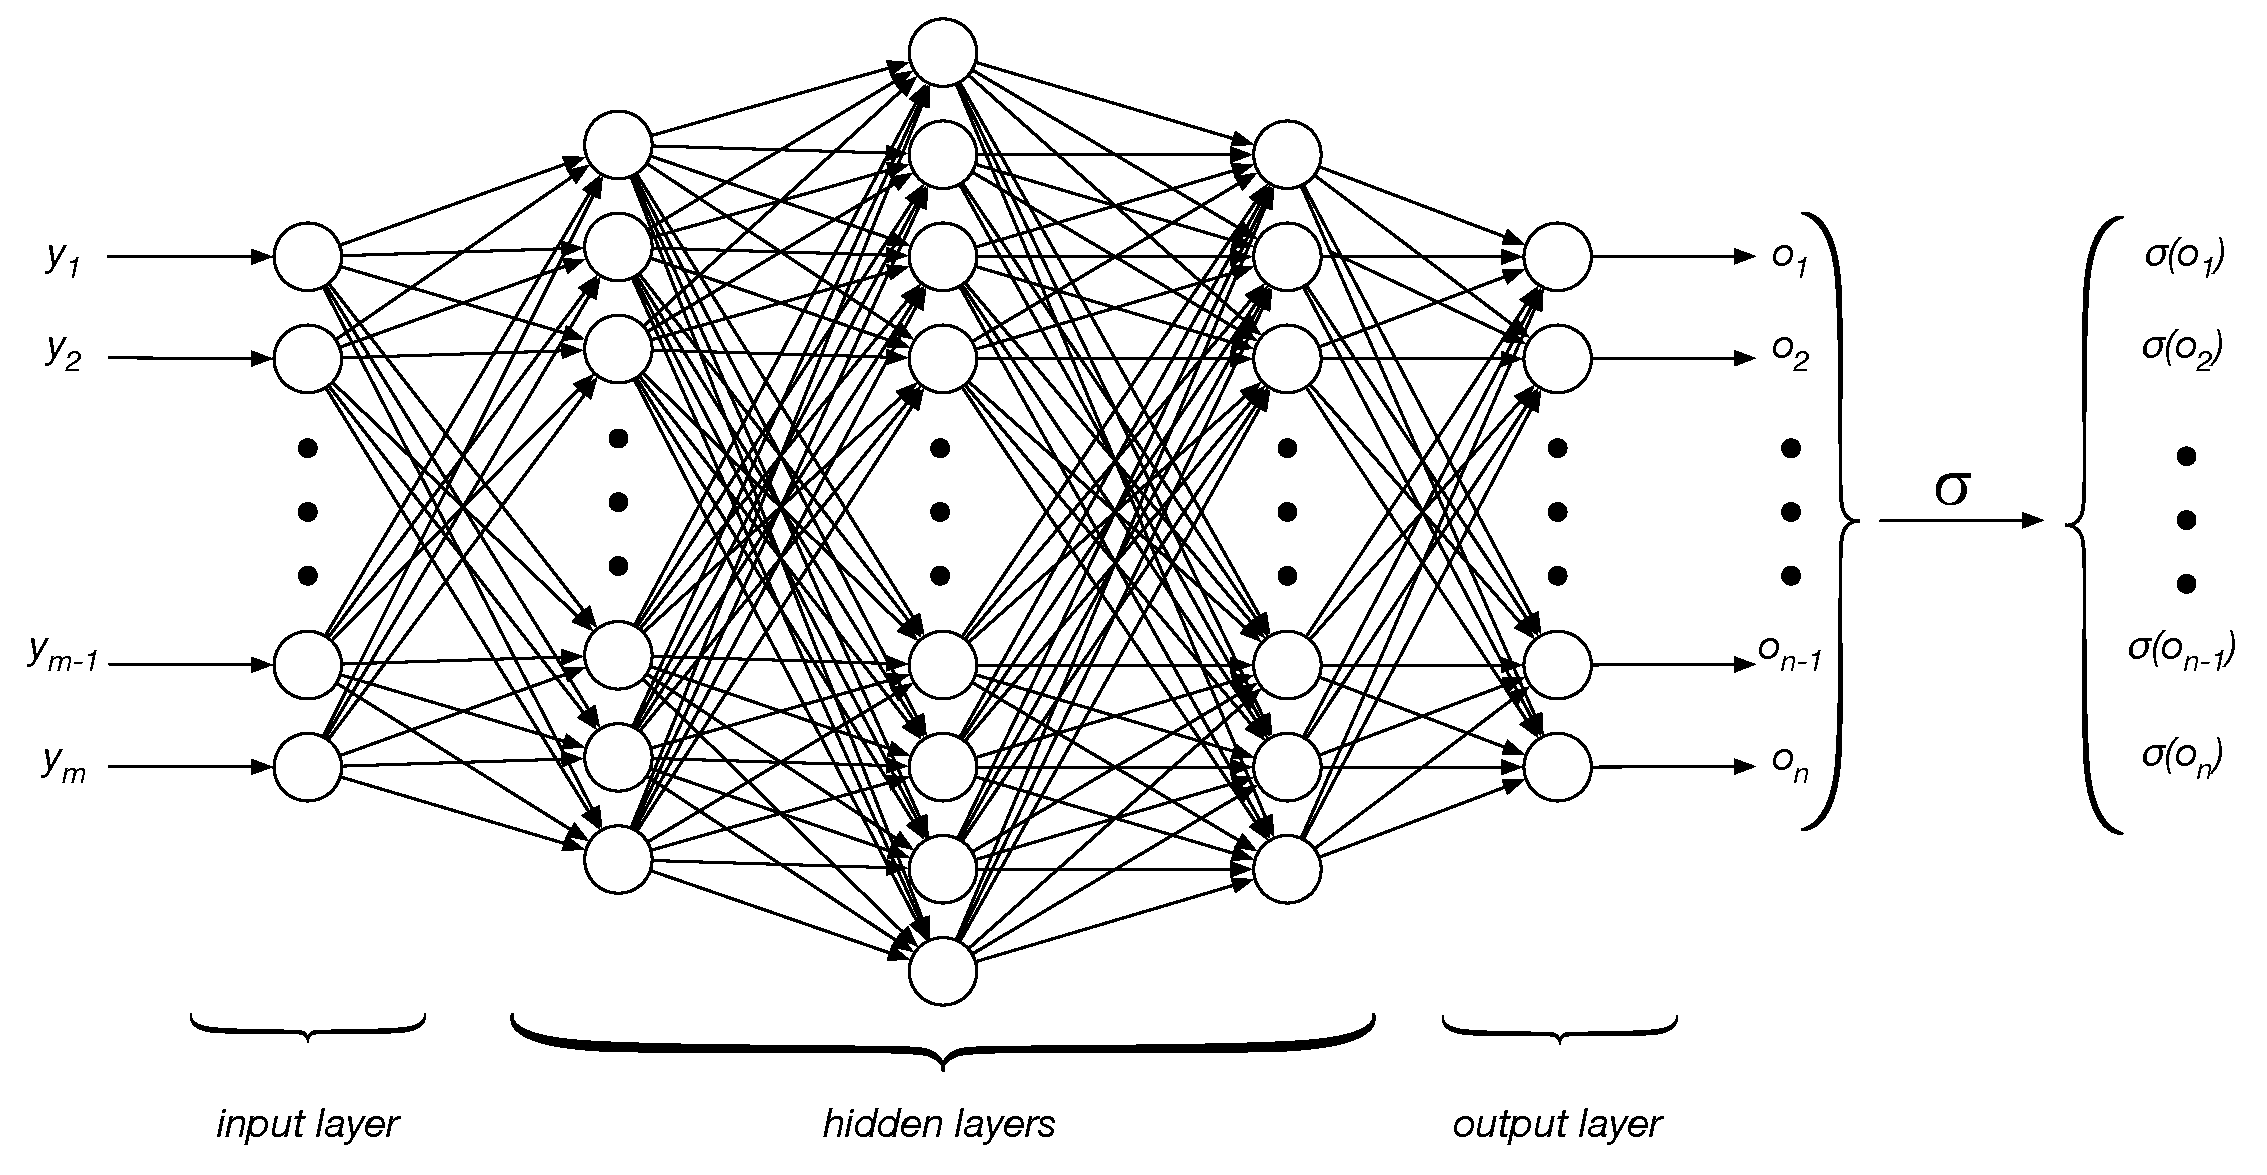
\includegraphics[ width=1.1\textwidth]{nn_struct.eps}
		\caption{Architecture of the neural network: $m$ is the number of sensors, i.e. the size of the observation's space, whereas $n$ the number of the recorded activities, i.e. the state's space.}
		\label{fig:ann_struct}
	\end{figure}
	\subsubsection{HMM}
	The HMM structure is usually defined by three matrices: $\pi$, which provides the a-priori probabilities for each hidden state, $T$, which features the probabilities to transition from one hidden state to the other and  $O$, the emission probabilities' matrix. In the hybrid model, $\pi$ and $T$ are generated by computing the frequencies of states and transitions in the training set, respectively. $O$ is not defined since its columns are computed at each step by the neural network, when they are needed. 
	\subsection{Viterbi algorithm}
	The implementation of the Viterbi algorithm required just a slight variation to work with our hybrid model: rather than accessing an emissions' probabilities' matrix for each elements of the observation sequence, our algorithm calls the trained neural network using the given configuration of sensors as input and uses its output in the forward step like if it was the column of the $O$ matrix associated with the given observation.
	
	\section{Implementation details}
	\subsection{System's architecture}
	Our system is composed by three main elements:
	\begin{enumerate}
		\item the cross-validator, which we'll describe later,
		\item the data parser,
		\item the hybrid model.
	\end{enumerate}
The hybrid model presents three static functions: one to encode features and target for the neural network (using a one-hot encoding for the target), one to compute the error of the hybrid model and one to compute the transition matrix based on the frequencies of transitions detected in the training set. Inside the class HybridHMM four functions:
\begin{enumerate}
	\item the constructor,
	\item the training function for the neural network,
	\item the test function for the hybrid model itself,
	\item the decode function, which implements the modified Viterbi algorithm for the hybrid HMM.
\end{enumerate}
	\subsection{Third-party libraries}
	We used \tt sklearn\rm, \tt numpy \rm and \tt pandas \rm for scientific computing matters. In particular, the \tt sklearn\rm provides a useful API, named \tt metrics\rm, that computes accuracy, precision and other model's evaluating values by simply feeding it the list of predictions and targets. The neural network was developed with \tt keras\rm, a high-level API which uses \tt tensorflow \rm as its back-end. 
	 	\begin{figure}
		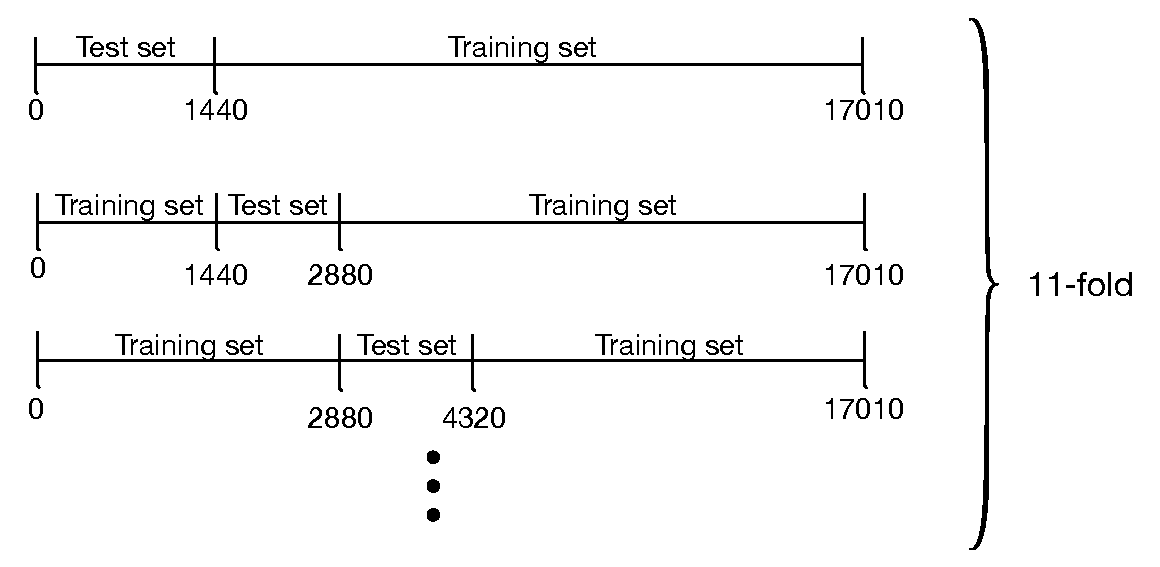
\includegraphics[ width=1.1\textwidth]{cv.eps}
		\caption{Cross validation of dataset $A$.}
		\label{fig:cv}
	\end{figure}
	\section{Results}
	\subsection{Cross validation}
	In order to evaluate the performance of the hybrid model, we used the cross-validation technique: we splitted the whole dataset into $k$ equal subsets and performed $k$ rounds of learning and testing: on each round $\frac{1}{k}$ of the data is held out as a test set and the rest of the dataset is used as training set. The basic idea is that each example plays a double role: both as test data and training data.
We used a one-day $k$-fold cross validation, in which the test set consisted of a sequence of $\thicksim 1440$ observations, the equivalent of an entire day divided by the time segments of $60$ seconds. Figure \ref{fig:cv} shows how the cross-validation was used with the dataset $A$: since $\thicksim 17000$ samples were generated during the parsing, the number of folds is $k = \floor{17000/1440} = 11.$	

\subsection{Data results}
	Thanks to the elimination of noise in the dataset and the deep neural network contribute, we obtained predictions with a pretty nice accuracy. We kept track of the average error of  both the neural network and the hybrid model. Since the neural network works on single instances at a time, we suspected that it would have outputted more accurate predictions than the hybrid model, which works on sequences of $\thicksim 1440$ elements at a time. As figure \ref{figure:err_graph} shows, we weren't so much wrong. Here, the error was computed simply by dividing the non-matching states in the sequence by the sequence's length, for each of the $\thicksim 10$ folds. The average error among all $k$-folds is:\\
	\begin{center}
		\csvautotabular{csvs/total_mean_errors.csv}
	\end{center}
i.e. the hybrid model has an average accuracy that is greater than $90\%.$
	\begin{figure}
		\centering
		\subfigure[Dataset $A$.]{\label{fig:err_graph_A}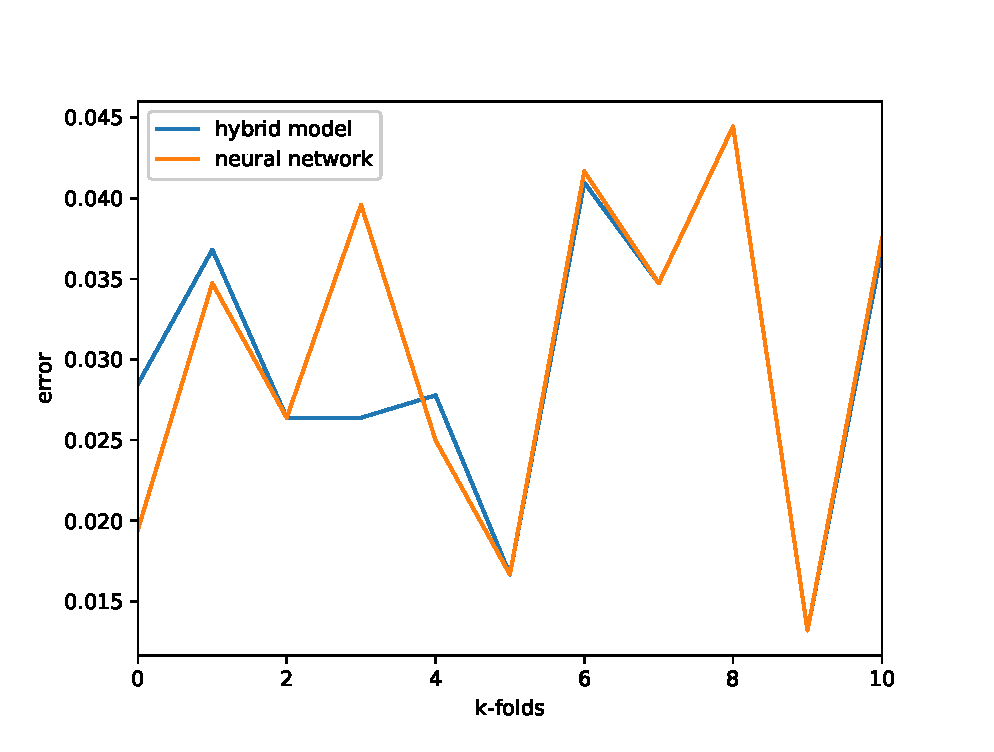
\includegraphics[width=0.49\textwidth]{A/errs.eps}}
		\subfigure[Dataset $B$.]{\label{fig:err_graph_B}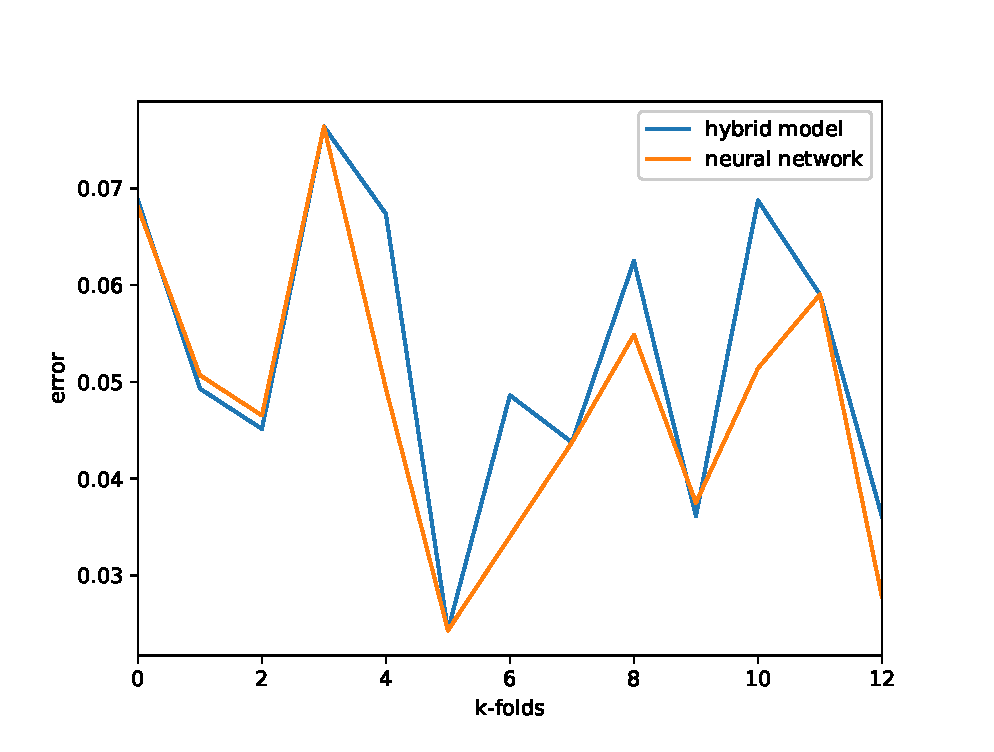
\includegraphics[width=0.49\textwidth]{B/errs.eps}}
		\caption{Mean error during testing.}
		\label{figure:err_graph}
	\end{figure}
	
	Figure \ref{fig:samples} shows graphically the mismatches in the first two folds for both dataset $A$ and $B$. If the prediction matches the target, the prediction's blue line is completely overlapped by the target's orange line. When a mismatch occurs, the blue line is not overlapped and can be seen. Here are presented the final results on evaluations related to the confusion matrix. Other than accuracy, we measured precision, recall and f measure:
	\begin{center}
		\csvautotabular{csvs/final_results.csv}
	\end{center}

	\subsection{Conclusion}
	Hybrid models have been researched and used extensively in the field of machine learning. Even in a small project like this one, we had the chance to see with our own eyes the power of deep learning and hybridization. Hybrid machine learning models have a wide range of possible application from medical research to social networks-related data analysis and many more. Deep convolutional neural networks models are even used to predict the form of black holes by feeding images of celestial objects as training data\cite{DBLP:journals/corr/GeorgeH17}: we are looking forward to see what new breakthroughs machine learning will lead to.
		\begin{figure}
		\centering
		\subfigure[$0$-th fold, dataset $A$.]{\label{fig:fold_0A}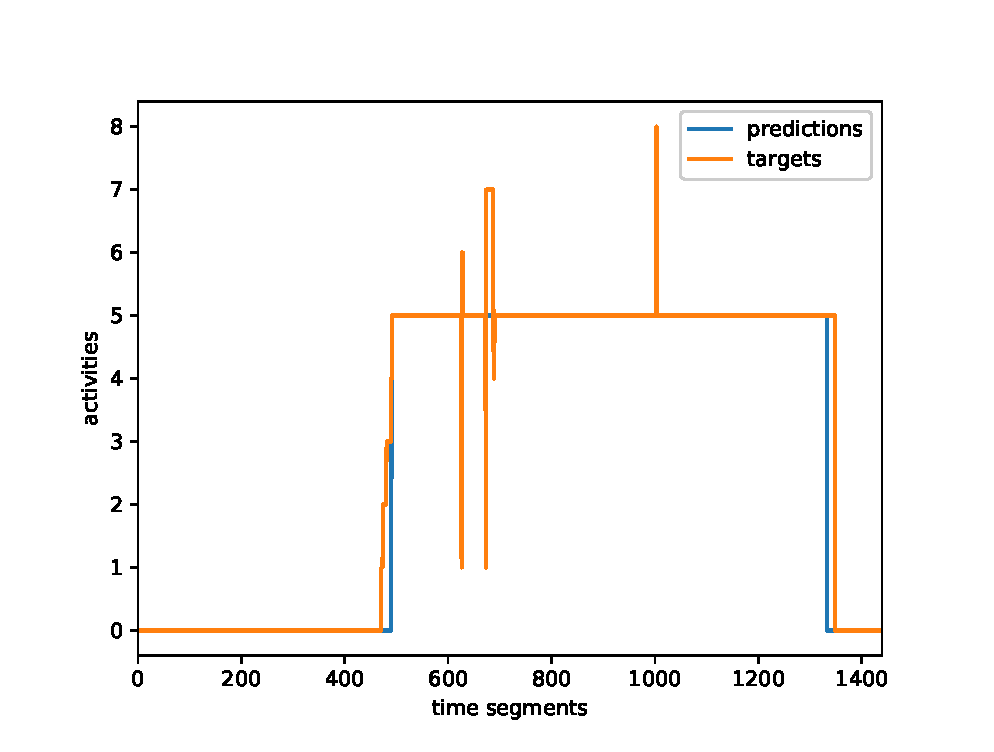
\includegraphics[width=0.49\textwidth]{A/predtarg_ratio/plot_of_0-th_fold.eps}}
		\subfigure[$1$-th fold, dataset $A$.]{\label{fig:fold,_1A}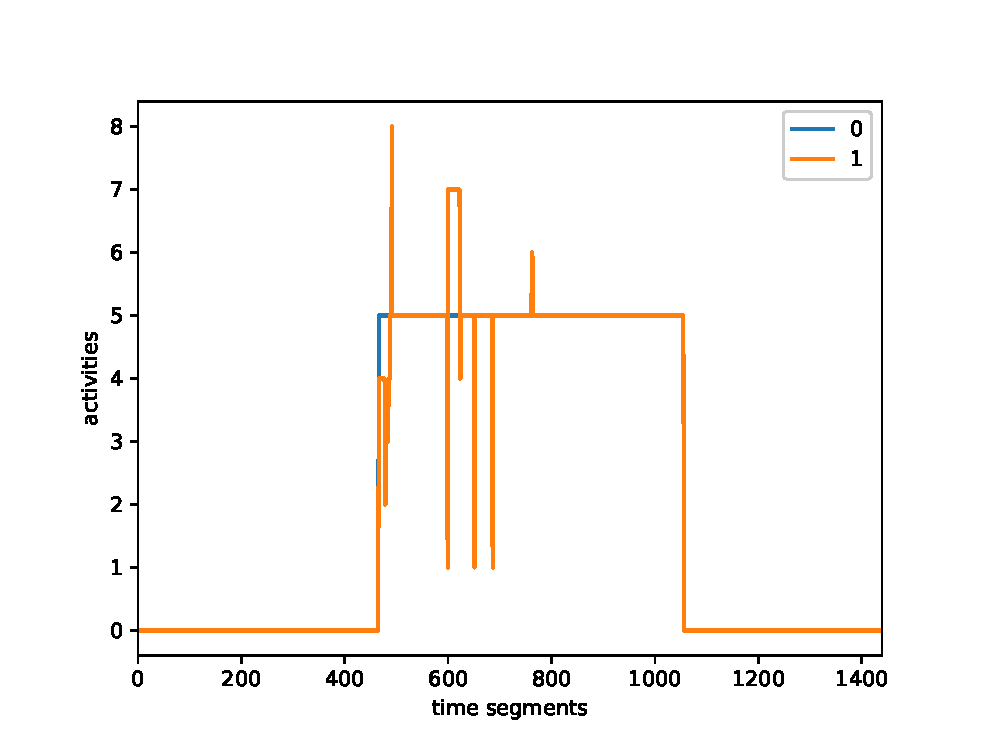
\includegraphics[width=0.49\textwidth]{A/predtarg_ratio/plot_of_1-th_fold.eps}}
		
		\subfigure[$0$-th fold, dataset $B$.]{\label{fig:fold_0B}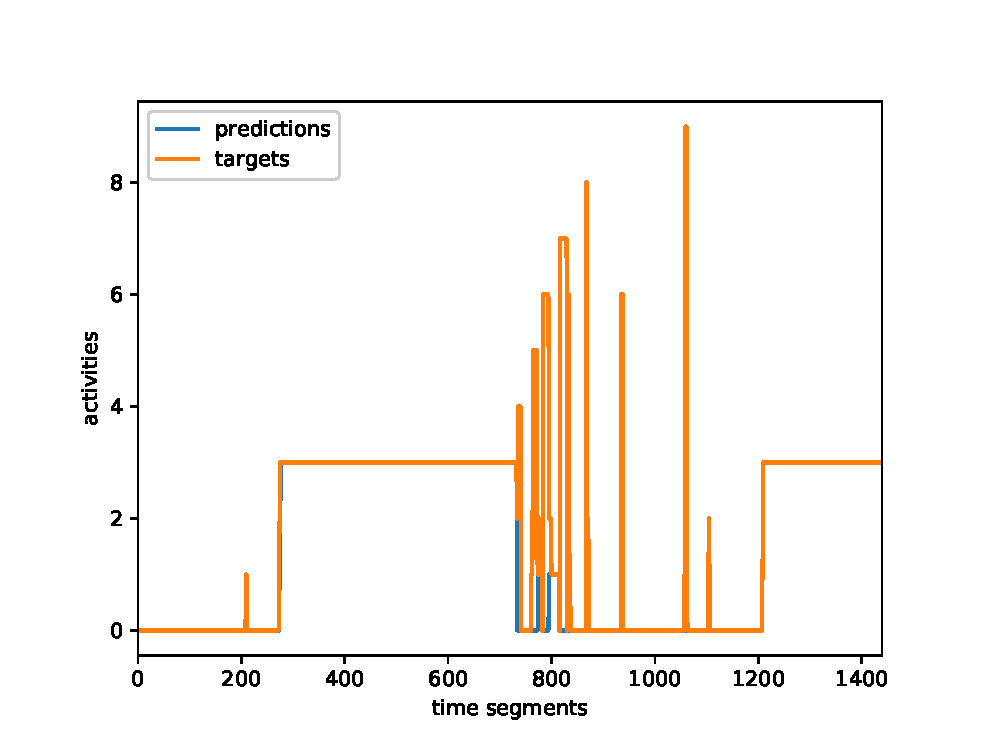
\includegraphics[width=0.49\textwidth]{B/predtarg_ratio/plot_of_0-th_fold.eps}}
		\subfigure[$1$-th fold, dataset $B$.]{\label{fig:fold,_1B}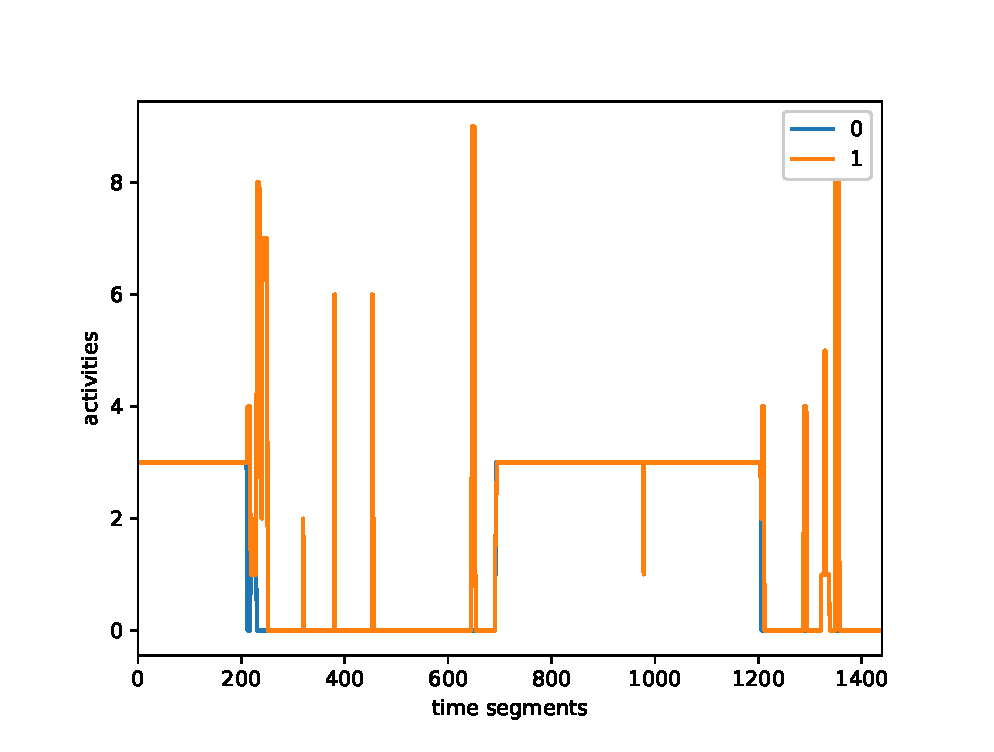
\includegraphics[width=0.49\textwidth]{B/predtarg_ratio/plot_of_1-th_fold.eps}}
		
		\caption{Prediction vs target mismatches.}
		\label{fig:samples}
	\end{figure}
	\newpage
	\bibliographystyle{plain}
	\bibliography{chapters/bibliography}
\end{document}